\section{Principle}
The second feature extraction method we used during this internship was AutoEncoder \cite{Rumelhart:1986:LIR:104279.104293}. Autoencoder (AE) is an unsupervised neural network algorithm that takes a signal as input and tries to reconstruct the same signal as the output. Generally, AE is composed of three parts (see figure \ref{fig:AE} \footnote{We take the convention in the figure that all circles can be anything such as Conv2D + Pooling, Dense, \dots}):
\begin{itemize}
 \item Encoder 
 \item Latent Space Representation (Red box in figure \ref{fig:AE})
 \item Decoder
\end{itemize}
 
\begin{figure}[h]
 \centering
 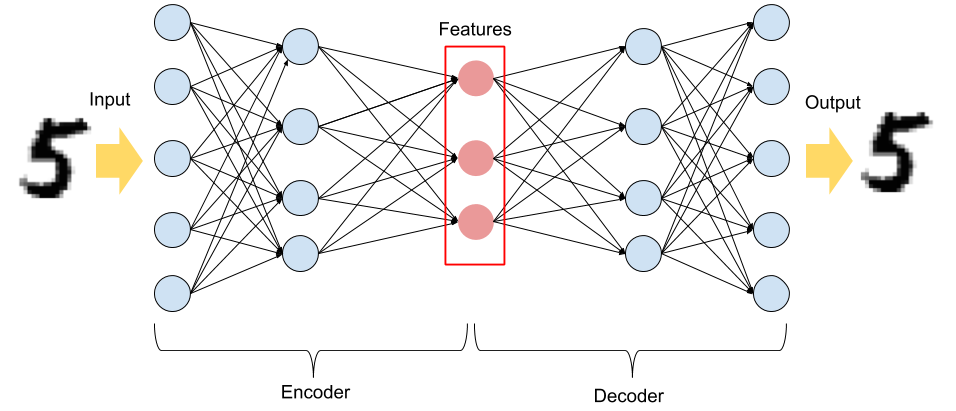
\includegraphics[scale=0.5]{AutoEncoder.png}
 % AutoEncoder.png: 956x411 px, 72dpi, 33.73x14.50 cm, bb=0 0 956 411
 \caption{Basic architecture of AutoEncoder}
 \label{fig:AE}
\end{figure}
Encoder and Decoder part work in the same way as a simple artificial neural network: a Feed Foward propagation algorithm to get the output from the input and Backward propagation of the error from the output to the input. The main difference with an artificial neural network is the Latent Space Representation which is typically a hidden layer located between the encoder and the decoder, with fewer neurons than any layers in Encoder or Decoder.\\
After the training, AutoEncoder can encode a certain set of data with less dimensionality than the input. It widely uses for feature extraction, segmentation, deconvolution, colorization, denoising,\dots\\
During the internship we tried two main architectures of AutoEncoder:
\begin{itemize}
 \item Sparse AutoEncoder, which has approximately the same behavior the Sparse Coding.
 \item Label Consistent AutoEncoder, which is a model we proposed based on the idea of Label-Consistent Sparse Coding.
\end{itemize}

\section{Sparse AutoEncoder}
In the respect of \textit{Sparseland} assumptions, \cite{DBLP:journals/corr/MakhzaniF13} introduced the K-Sparse AutoEncoder. The goal is the same as Sparse Coding, we want to compute a sparse representation from an input signal but the method is different. Here we do not have the dictionary directly, we have an Encoder that finds the sparse representation for us using artificial neurons or convolution blocks.\\
To allows the Autoencoder to find this sparse representation we must add a term in the loss function. It is called a regularizer, which is applied to the last layer of our encoder. We decided to keep using the $l_1$ norm for this regularizer.\\ 
Unlike the traditional Sparse Autoencoder, we decided to use more hidden units at the end of the encoder (cf figure \ref{fig:SAE}). With this addition, we create a discriminative representation instead of compressive representation.\\
\begin{figure}[h]
 \centering
 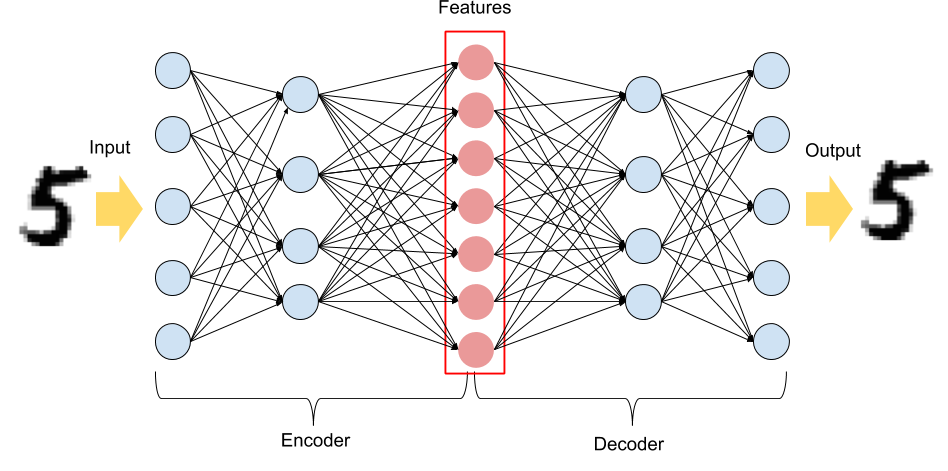
\includegraphics[scale=0.5]{sparse_AutoEncoder.png}
 % sparse AutoEncoder.png: 948x471 px, 72dpi, 33.44x16.62 cm, bb=0 0 948 471
 \caption{Example of Sparse AutoEncoder architecture}
 \label{fig:SAE}
\end{figure}

\newpage
\section{Labels Consistent AutoEncoder}
We proposed a new Autoencoder model for extraction of discriminative features. For this model, we were inspired by the Label-Consistent Sparse Coding and especially the Q matrix. Our idea is to bring the information on the label by encouraging the use of certain filters for a class.\\
However, we also want to keep the reconstruction. To achieve these two objectives, we decided to create two parallel branches, one for each problem (we show an example of our model architecture in figure \ref{fig:LC_AE}).\\
We called this model \textit{Label Consistent AutoEncoder}.  To fit with our previous studies  (especially CSC's method) we also use convolution blocks and pooling blocks for encoding, convolution and upsampling for decoding and dense block for the label consistent term.\\
We also tested this model with the Sparsity constraint to see if it would improve the results. We called this model \textit{Labels-Consistent Sparse Autoencoder}.\\
\begin{figure}[h]
 \centering
 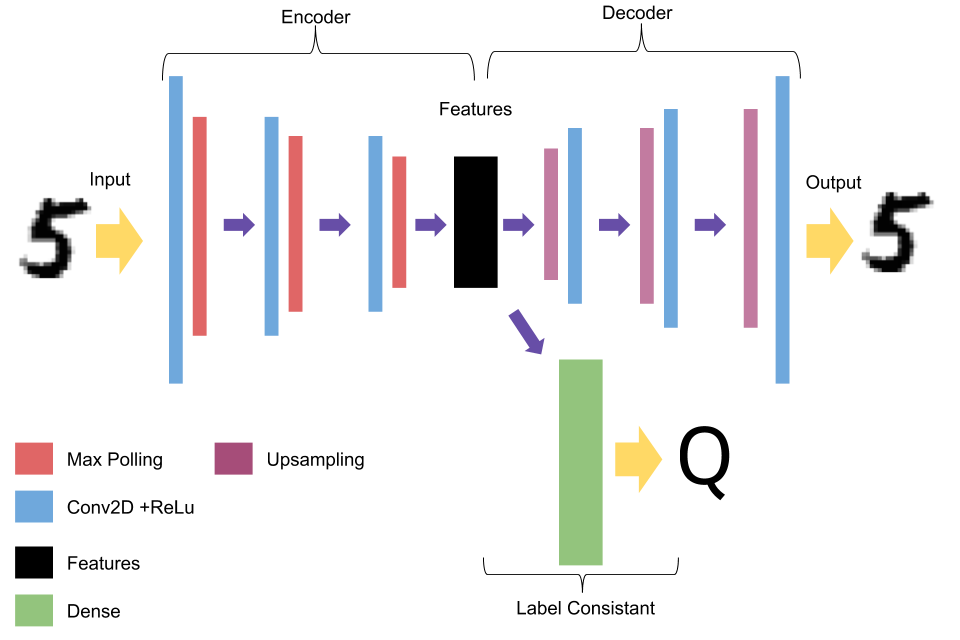
\includegraphics[scale=0.5]{LC_AutoEncoder.png}
 % LC_AutoEncoder.png: 964x627 px, 72dpi, 34.01x22.12 cm, bb=0 0 964 627
 \caption{Example of Label Consistant Autoencoder architecture}
 \label{fig:LC_AE}
\end{figure}
In addition, we train a A matrix in the same way as we did for $A_0$ in the LC-KSVD and multiply this A matrix with the features to get a more discriminative representation.
\newpage
\section{Experimentation details}
\subsection{Application of different Autoencoder on MNIST}
\subsubsection{K Sparse Autoencoder}
\begin{figure}[h]
 \centering
 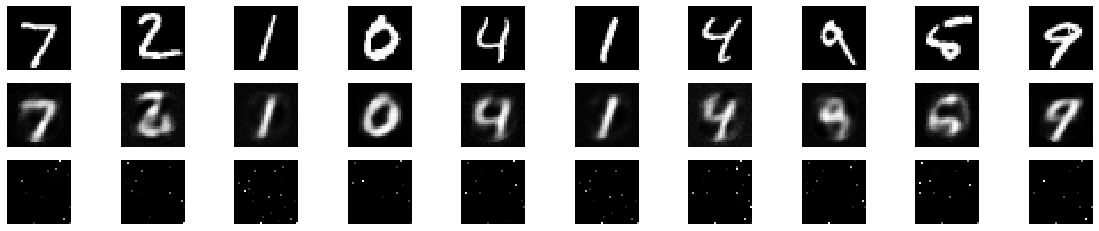
\includegraphics[scale=0.4]{SAE.png}
 % SAE.png: 1130x230 px, 72dpi, 39.87x8.12 cm, bb=0 0 1130 230
 \caption{Reconstruction using decoder and encoded data}
 \label{fig:SAE_result}
\end{figure}

\begin{figure}[h]
 \centering
 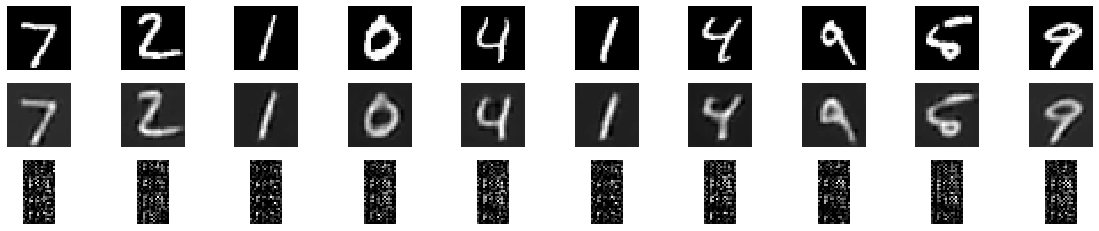
\includegraphics[scale=0.4]{KSparseAE_CONV.png}
 % KSparseAE_CONV.png: 1099x231 px, 72dpi, 38.78x8.15 cm, bb=0 0 1099 231
 \caption{K Sparse Autoencoder using convolution, pooling, upsampling results}
 \label{fig:SAEconv}
\end{figure}
Here, we see that reconstruction is better in the context of convolution utilization (figure \ref{fig:SAEconv}) rather than with dense (figure \ref{fig:SAE}). This is explained by the fact that the method with Dense has only one layer whereas the method with convolution is deeper.
\subsubsection{Labels Consistent Autoencoder}
\begin{figure}[h]
 \centering
 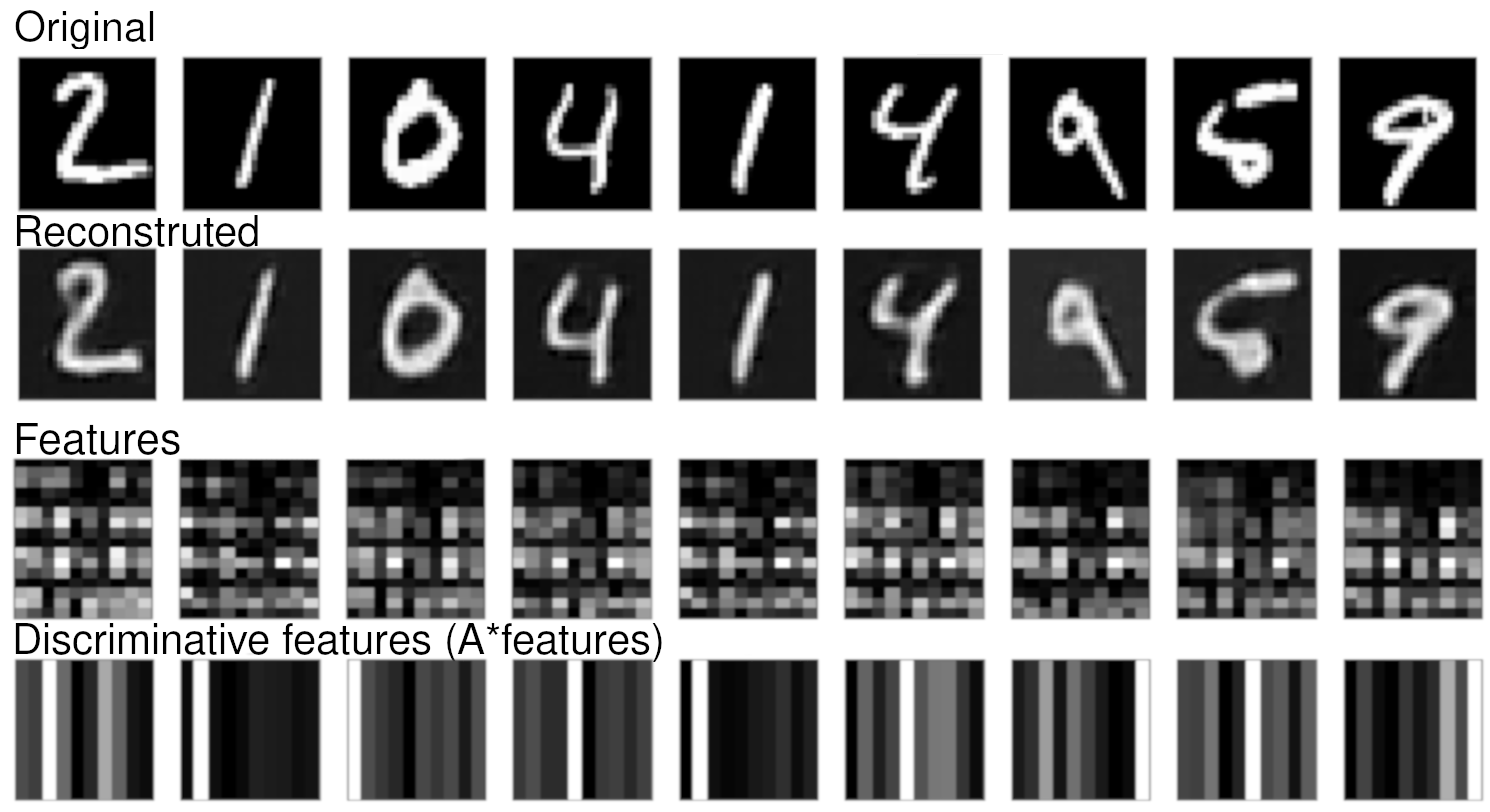
\includegraphics[scale=0.3]{LCAE.png}
 % LCAE.png: 1490x812 px, 100dpi, 37.85x20.62 cm, bb=0 0 1073 585
 \caption{MNIST samples with the  LC-Autoencoder}
 \label{fig:LCAE}
\end{figure}
\subsubsection{Label Consistent Sparse Autoencoder}
\begin{figure}[h]
 \centering
 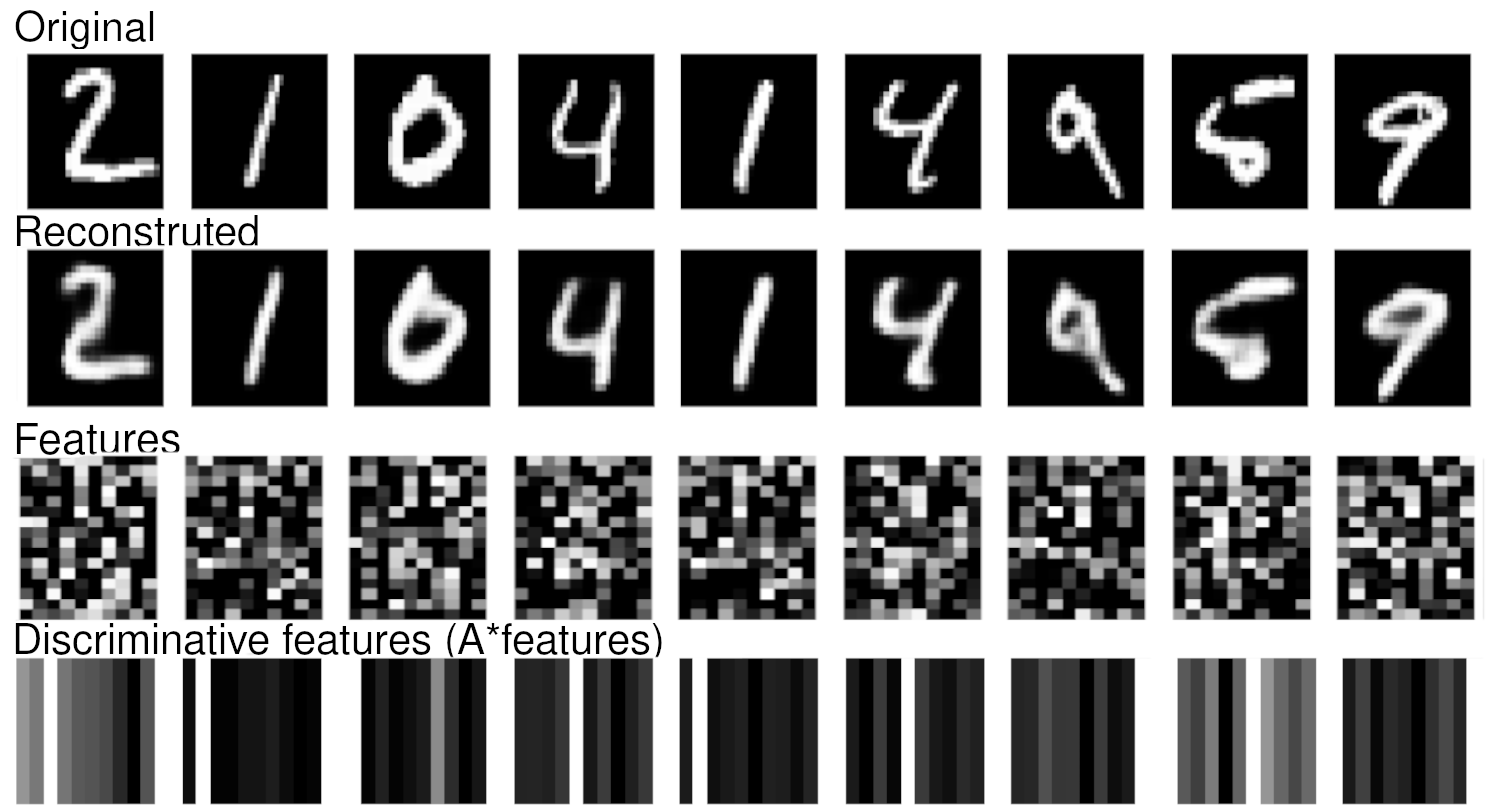
\includegraphics[scale=0.3]{Sparse-LCAE.png}
 % Sparse-LCAE.png: 1490x812 px, 100dpi, 37.85x20.62 cm, bb=0 0 1073 585
 \caption{MNIST samples with the Sparse LC-Autoencoder}
 \label{fig:SLCAE}
\end{figure}
In figure \ref{fig:LCAE} and figure \ref{fig:SLCAE} we can see that there is a good reconstruction but especially that the discriminating features $A*Features$ are perfect for classification, indeed, there is a white band at a precise location depending on the number label.
\subsection{Classification for Autoencoder}


\begin{center}
\begin{tabular}{|c|c|c|}\hline
× & \textbf{SVM accuracy} & \textbf{K-means accuracy}\\\hline
\textbf{K Sparse AE (Dense)} & 0.91 & 0.22\\\hline
\textbf{K Sparse AE (Conv with 32 filters)} & 0.96 & 0.19\\\hline
\textbf{K Sparse AE (Conv with 10 filters)} & 0.95 & 0.23\\\hline
\textbf{Label Consistent AE} & 0.98 & 0.98\\\hline
\textbf{LC Sparse AE} & 0.98 & 0.98\\\hline
\end{tabular}
\end{center}
It is clear that the results of the different autoencoders are good when using an SVM as a classifier. Nevertheless, the addition of the Label Consistency branch allows a clear improvement both on the SVM but also on the K-means, going to classification results of over 98\%. 
